\newpage
\section{Digits Classification with K Nearest Neighbors (45 points)}

\subsection{Task \#1}

\paragraph{How does $n$ affect fluctuation in validation error?}~\smallskip

\begin{figure}[H]
  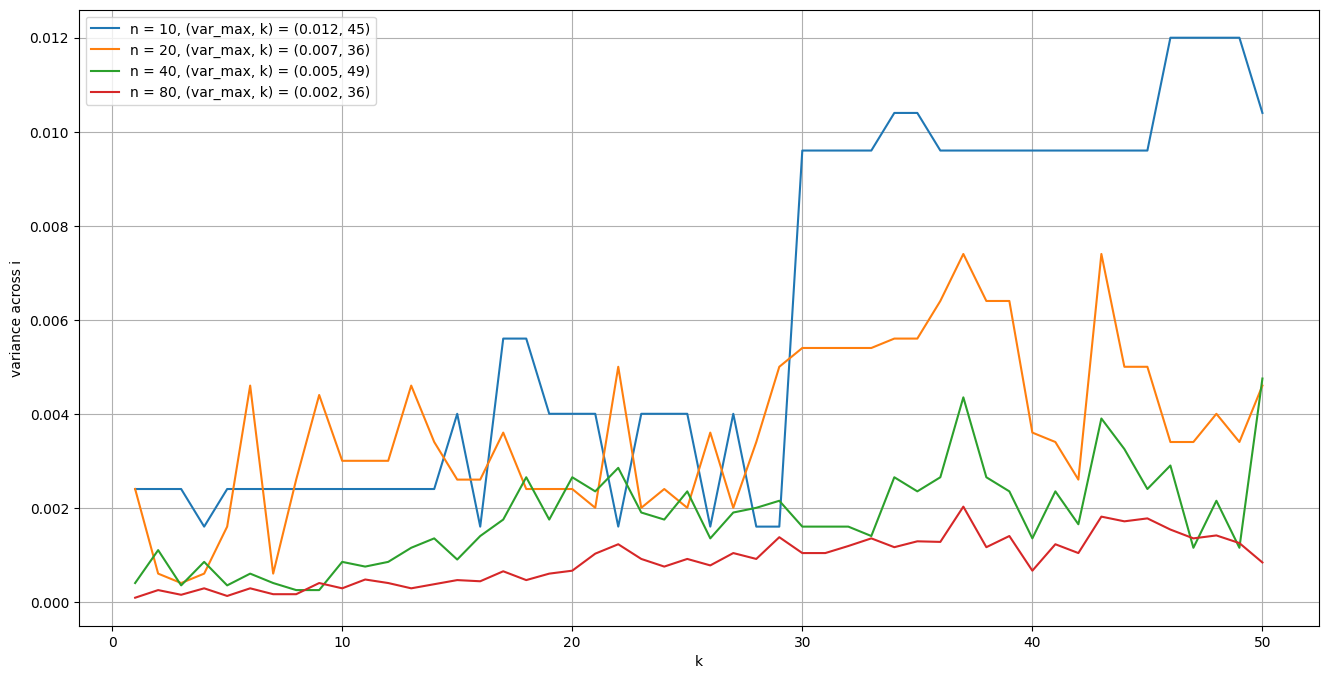
\includegraphics[width=\textwidth]{figures/fig2_2.png}
\caption{\footnotesize \it Fluctuation in validation error for varying i as a function of k, for
  each n.}
\label{fig:2-2}
\end{figure}

While $i$ determines which subset of the data is used for validation, $n$
determines the \textit{size} of each of these validation subsets.

There is a very clear trend in the relationship the value of $n$ and fluctuation
in validation error across all values of $k$, but it is best illustrated by
examining the right end of the plot.

For high values of $k$ (roughly 30 and greater), there is an undeniable
indication that the higher the value of $n$, the smaller the fluctuation in
validation error across values of $i$. This is because as $n$ increases, the
differences between two given validation subsets are smoothened out -- in other
words, the smaller the $n$, the more the result is influenced by outliers in the
validation set.


\newpage
\paragraph{How does $K$ affect prediction accuracy?}~\smallskip

\begin{figure}[H]
  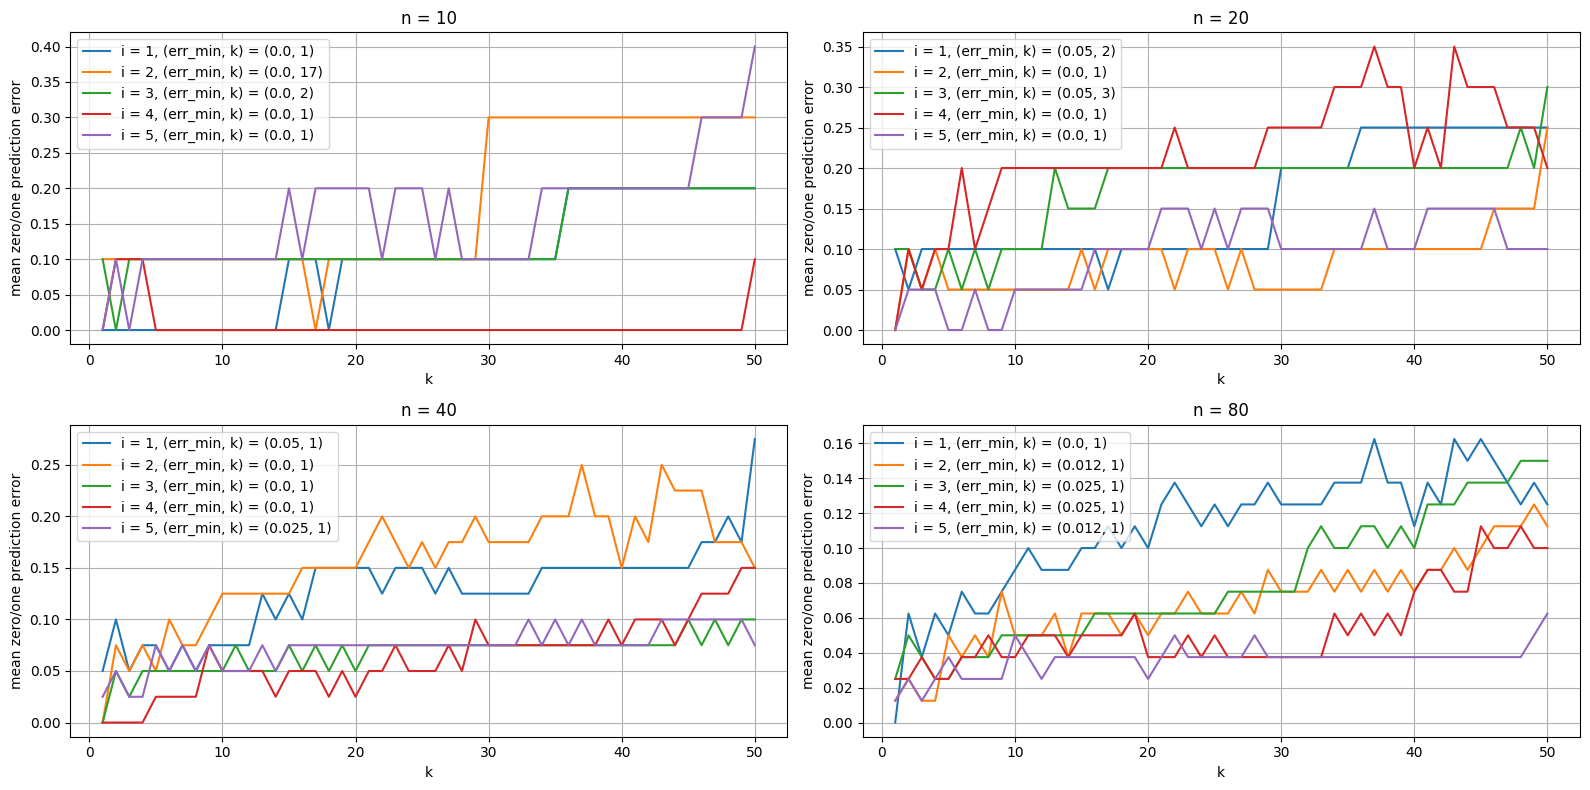
\includegraphics[width=\textwidth]{figures/fig2_1.png}
  \caption{\footnotesize \it Mean zero/one prediction error of KNN for varous i, n, k.}
\label{fig:2-1}
\end{figure}

Interestingly, the overall best $K$ seems to be $K^* = 1$, with almost zero
validation error for most values of $i$ across all $n$.

For all four values of $n$, prediction error seems to increase with $K$. This is
likely because our training set is only 100 digits, and as $K$ increases towards
half of the training set, the model moves closer towards simply estimating the
sample mean.


\subsection{Task \#2}

\begin{figure}[H]
  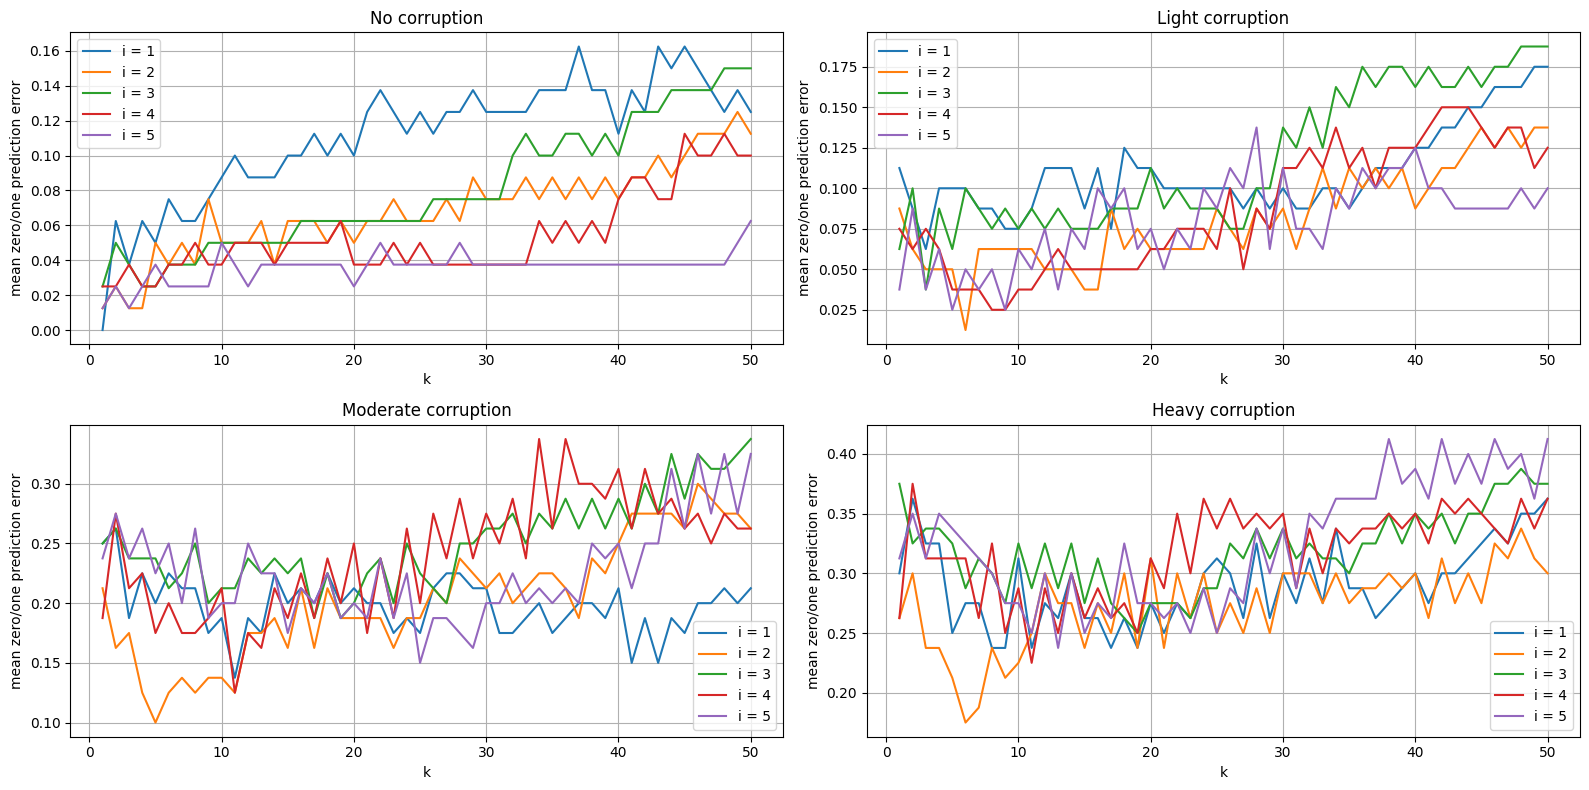
\includegraphics[width=\textwidth]{figures/fig2_3.png}
\caption{\footnotesize \it Mean zero/one prediction error of KNN for various degrees
         of data corruption; for n = 80 and varying i, k.}
\label{fig:2-3}
\end{figure}

\paragraph{How does corruption magnitude influence prediction accuracy and the optimal
value of K?}~\smallskip

Not surprising, there is a correlation between corruption magnitude and
prediction error -- for the uncorrupted set, the prediction error lies roughly
in the range $[0, 0.16]$, while prediction errors lie roughly in the ranges
$[0.02, 0.18]$, $[0.1, 0.3]$, and $[0.2, 0.4]$ for the lightly, moderately, and
heavily corrupted sets, respectively. For the heavily corrupted set, prediction
error reaches as high as roughly 40\% for $i = 5$.

As far as the optimal $K$, based on the plots we may still be inclined to simply
choosing small values of $K^*$ for the three corrupted sets, but the indication
is not as strong based on the plots alone, since the trend in the curves seem
flatter than that of the uncorrupted set -- this perhaps applies less so for the
lightly corrupted set.

Most interestingly, however, is perhaps the fluctuation in validation error
across values of $i$. This has not been examined explicitly, but for the heavily
corrupted set it appears as though the five curves stick closer together than
for the uncorrupted set.

\sectend
